\graphicspath{ {4-NoSQL/} }
\chapter{Banco de Dados NoSQL}
\label{nosql}

O desenvolvimento de novas aplicações e surgimento de novas soluções 
para sistemas gerou crescimento no volume de dados de maneira acelerada. 
Com isso cresce também o número de usuários, necessitando portanto escalar 
o banco de dados. Existem duas soluções para escalar um sistema: o 
escalonamento vertical, que consiste em um \textit{upgrade} do servidor no 
qual o banco está hospedado; e o horizontal, aumentando o número de 
servidores e distribuindo o banco \cite{pritchett2008base, sharding2018educative}. 

Existem algumas desvantagens no \textit{upgrade} de um sistema. 
O banco de dados pode superar a capacidade da melhor configuração 
disponível no mercado, e ainda é caro por requerer a aquisição de 
uma configuração melhor. Mesmo considerado mais complexo, o 
escalonamento horizontal é mais viável. Entre as soluções apresentadas 
no particionamento horizontal em banco de dados estão o particionamento funcional e o 
\textit{sharding} \cite{pritchett2008base}. 

O particionamento funcional consiste em fragmentar os dados de acordo 
com a forma como são utilizados dado um contexto. Um esquema com quatro entidades, 
\textit{usuários}, \textit{produtos}, \textit{clientes} e \textit{endereço} 
pode ser distribuído em quatro servidores, 
um para cada entidade. Entidades que são utilizadas somente para leitura podem 
ser separadas de entidades onde dados são escritos, caracterizando outro 
exemplo de particionamento funcional. O problema com esta estratégia está 
no acoplamento entre entidades: se duas ou mais entidades estiverem 
relacionadas elas deverão estar no mesmo servidor, caso contrário não 
será possível atribuir as restrições de chave àquele relacionamento \cite{pritchett2008base}. 
Tomando o exemplo acima com as quatro entidades, supondo que \textit{cliente} 
e \textit{endereço} estejam relacionadas estas devem 
ser armazenados no mesmo servidor. 

A segunda estratégia, o \textit{sharding}, consiste em dividir os dados do banco 
utilizando algum critério de separação que não seja limitado à 
funcionalidade das entidades. Soluções como particionamento com base em 
\textit{hash} ou listas podem ser aplicadas. Considerando dez servidores e uma chave 
primária auto-incremental, a função de \textit{hash} pode tomar o módulo da chave 
primária pelo total de servidores como critério de seleção da partição 
na qual o dado será inserido. Utilizando uma lista é possível definir valores 
para os servidores e distribuir os dados de acordo com esses valores. 
Por exemplo, as linguagens C++, Java e C\# poderiam ser inseridas em uma 
partição destinada à linguagens orientadas a objeto.

O \textit{sharding} enfrenta problemas com junções entre dados, visto que os dados 
devem ser recuperados de diferentes partições e a maioria dos SGBDR não 
oferece suporte a chaves estrangeiras sob diferentes servidores, restando 
ao desenvolvedor tratar isso no código da aplicação \cite{pritchett2008base}. 
Uma solução para tais 
problemas é a denormalização de dados para que o número de junções diminua ou, 
no melhor dos casos e quando possível, seja zero. Contudo, isso é um problema 
para modelos relacionais, visto que trabalham sobre uma modelagem normalizada de dados. 
Além disso e de não se adaptarem à escalabilidade horizontal, 
são complexos e o fato de trazerem todas as informações de uma entidade sob a 
forma de tuplas causa lentidão em um ambiente analítico na recuperação de dados, 
cujas consultas percorrem o banco visando atributos específicos, processando 
somente o necessário. 

Outro problema crítico ao não utilizar a escalabilidade horizontal está na 
disponibilidade dos dados. Enquanto um banco se apoiar na escalabilidade vertical, 
qualquer queda no servidor acarretará na queda total no sistema de armazenamento, 
ao passo que quando se trabalha com servidores em paralelo a queda em uma máquina 
não trará prejuízos no conjunto todo. Assim, soluções como melhorar o hardware do 
servidor continuam sendo desvantajosas. Além da escalabilidade, disponibilidade 
de dados foi um dos argumentos utilizados por um dos engenheiros da rede social 
Twitter ao migrar do MySQL para o Cassandra, um SGBD NoSQL. 
Em 2008 a rede ficou fora do ar por 84h \cite{twitter2010}.

Com o intuito de suprir tais problemas de escalabilidade, disponibilidade 
e recuperação rápida de dados, entre 2004 e 2007 os SGBD NoSQL começaram 
a ganhar destaque com o surgimento das bases de dados BigTable da Google \cite{chang2008bigtable}, e Dynamo 
da Amazon \cite{decandia2007dynamo}. O termo NoSQL, embora a princípio pareça indicar total independência 
de SQL, significa \textit{Not Only SQL}, “Não Apenas SQL”. Também, ele não descreve um 
único tipo de SGBD, mas sim uma classe de modelos, cada qual com suas propriedades. 
As mais conhecidas são quatro:

\begin{itemize}
    \item{\textbf{Orientado a Grafos}}, que se utiliza da Teoria dos Grafos para estruturar seus dados. 
    Um exemplo desta classe é o Neo4j \cite{neo2018nosql}.
    \item{\textbf{Orientado a Chave-Valor}}, que armazena os dados de forma similar a uma tabela \textit{hash}, 
    com uma chave referenciando um valor, ou tipo de dado. Exemplos são o Project Voldemort \cite{voldemort2018nosql}, 
    DyanmoDB \cite{amazon2018nosql}, o Riak \cite{riak2018nosql} e o Redis \cite{redis2018nosql}.
    \item{\textbf{Orientado a Documento}}, uma versão melhorada do Chave-Valor, 
    no qual os valores são armazenados como documentos através de estruturas complexas como JSON e XML. 
    Exemplos são o MongoDB \cite{mongo2018nosql} e o CouchDB \cite{couch2018nosql}.
    \item{\textbf{Orientado a Colunas}}, ou modelo colunar, 
    que utiliza tabelas como armazenamento de entidades, 
    porém não agrupa os dados sob forma de tuplas, e sim colunas. Exemplos são o MonetDB \cite{monetdb2017c}, C-Store \cite{cstore2018nosql}, BigTable \cite{google2018nosql} e Cassandra \cite{cassandra2018nosql}.
\end{itemize}

De maneira geral, as vantagens no uso de um SGBD NoSQL estão no rápido processamento de um grande volume de dados, flexibilidade para expansão e baixo custo de escalabilidade. Devido ao vasto número de SGBD dentro de cada classe de NoSQL, esses bancos também podem ser classificados de acordo com o Teorema CAP (do inglês \textit{Consistency, Availability, Partition tolerance}). Segundo Eric Brewer \cite{brewer2000towards, gilbert2002brewer}, um sistema distribuído não é 
capaz de conciliar consistência, disponibilidade e tolerância a partição de dados simultaneamente, tendo que optar por apenas dois destes. 
SGBDR prezam por disponibilidade e consistência de dados seguindo o ACID, porém a preocupação com consistência 
pode tornar a manipulação de dados lenta. Visto que o movimento NoSQL surgiu com a intenção de 
melhorar a escalabilidade e disponibilidade de dados, e tornar a manipulação destes mais rápida, 
a maioria deles trabalha com os atributos de disponibilidade e tolerância à partição. 
Essa configuração assume um conceito diferente do ACID para bancos NoSQL, e Pritchett \cite{pritchett2008base} propôs um teorema diferente deste, mais otimista, onde a consistência é relaxada, o Teorema BASE (\textit{Basically Available, Soft State, Eventual Consistency}).

O Teorema BASE assume que a consistência em um banco 
de dados está em estado de fluxo, ao contrário do ACID que força a consistência a cada operação, 
sendo este considerado pelo autor um método pessimista. 
Neste cenário a disponibilidade é garantida devido à tolerância a partição, fazendo 
com que a falha de um servidor não cesse o funcionamento de todo o sistema -- por exemplo, caso uma partição falhe em um sistema rodando sobre dez servidores, apenas 10\% dos dados estarão indisponíveis e somente os usuários daquela partição serão afetados.


\section{Modelo de SGBD Colunar}

Dentre as categorias de bancos de dados NoSQL a que melhor se adequa aos 
propósitos analíticos é a colunar. Sistemas colunares armazenam seus dados 
em colunas que representam atributos das entidades, fazendo com que apenas os atributos necessários sejam 
lidos \cite{khoshafian1987query}, o que diminui o tempo de acesso 
ao disco \cite{matei2010column, abadi2008column}. Cada uma destas colunas pode armazenar seus valores utilizando o par 
\textit{chave, valor} \cite{abadi2013design, khoshafian1987query}, sendo esta uma das formas de implementação 
de um sistema colunar (descrita na Seção \ref{sec:implementacao_col} deste capítulo). 
A Figura \ref{fig:row-col} ilustra de forma simples, embora apenas visual, 
a diferença principal entre um armazenamento utilizando linhas, conforme a Figura \ref{fig:row}, e outro utilizando 
colunas, Figura \ref{fig:column}, a partir dos registros da Figura \ref{fig:regs}, baseada na entidade \textit{funcionário} apresentada no Capítulo \ref{sgbd}.

\begin{figure*}[htpb]
	\centering
		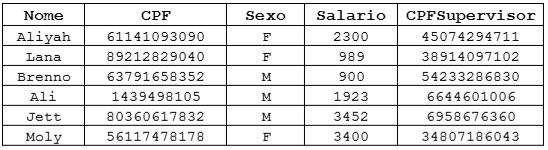
\includegraphics[width=12cm]{registros}
	\caption{Exemplos de registros para a entidade \textit{funcionário} apresentada no Capítulo \ref{sgbd}}
	\label{fig:regs}
\end{figure*}

\begin{figure*}[htpb]
    \centering
    \subfigure[]{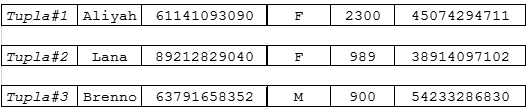
\includegraphics[width=8cm]{row}\label{fig:row}}
    \subfigure[]{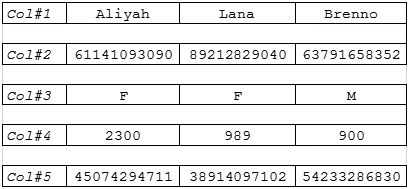
\includegraphics[width=6.8cm]{column}\label{fig:column}}
    \caption{Diferença visual entre registros armazenados em um banco relacional e colunar}
    \label{fig:row-col}
\end{figure*}

Matei \cite{matei2010column} cita algumas vantagens de sistemas colunares:

\begin{itemize}

    \item{\textbf{Melhor desempenho}}, pela forma com que os dados são armazenados e o uso de índices 
    visando o armazenamento ao invés de localização de registros, resultando em menos operações de 
    entrada e saída.
    \item{\textbf{Rápidas operações de agrupamento}}, bastante utilizadas em ambientes OLAP, visto 
    que valores de um mesmo atributo são armazenados consecutivamente. Bem como operações matemáticas, 
    como recuperar o maior ou menor valor, soma e média.
    \item{\textbf{Alta compressão de dados}} pode ser alcançada, devido às chances de se ter 
    valores repetidos para um mesmo atributo serem maiores.

\end{itemize}

Existem diferentes abordagens para se implementar um SGBD colunar. Essas abordagens levam em conta 
mudanças na codificação de um banco, apenas na modelagem dele, bem como se será possível atingir 
níveis altos de compressão. A primeira técnica consiste no \textbf{particionamento vertical} dos dados, a 
segunda em \textbf{modificar a camada de armazenamento} e a terceira corresponde a junção de ambas.

\section{Implementação do Sistema Colunar}
\label{sec:implementacao_col}

Antes de detalhar os métodos de implementação de um banco de dados colunar, é fundamental discutir sobre a reconstrução de tuplas nesse tipo de SGBD. 
Segundo Abadi et al. \cite{abadi2007materialization}, a parte lógica e visual de um banco de dados colunar se apresenta da mesma forma que 
um relacional. Isso faz com que a maioria dos SGBD colunares ofereçam uma interface relacional de comunicação, compatível com os padrões.

Como os atributos de um modelo colunar acabam ficando separados em disco um do outro, eles precisam ser unidos novamente em tuplas para 
que o resultado de uma consulta seja exibido. Existem duas técnicas para realizar essa reconstrução, ou materialização: \textit{Early Materialization} (EM) e 
\textit{Late Materialization} (LM) \cite{abadi2007materialization, abadi2008query}.

A técnica de \textit{Early Materialization}, melhor traduzida como materialização prévia nesse contexto, é a política adotada por banco de dados relacionais, e consiste 
em adicionar as colunas à tupla conforme a coluna é requisitada na consulta. Essa técnica não leva em conta o predicado da consulta, isto é, considere 
a consulta a seguir:

\begin{lstlisting}[language=SQL,label=sql_1]
                    SELECT nome FROM funcionario 
                    WHERE salario >= 1000 AND sexo='F'
\end{lstlisting}

A EM irá processar essa consulta e construir uma tupla com os atributos \textit{nome, salário} e \textit{sexo}, com todos os registros 
armazenados em banco. Considere que os registros são como mostrados na Figura \ref{fig:regs}, o construtor de tuplas retornará os registros conforme a Figura \ref{fig:em}. Esse método só analisa o predicado após a construção das tuplas, o que não acontece na LM. 

\begin{figure*}[htpb]
	\centering
        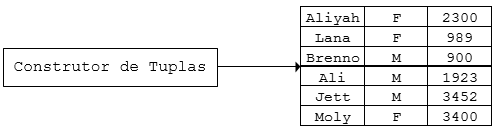
\includegraphics[width=14cm]{em}
	\caption{Tuplas reconstruídas a partir da \textit{Early Materialization}}
	\label{fig:em}
\end{figure*}

\begin{figure*}[htpb]
	\centering
        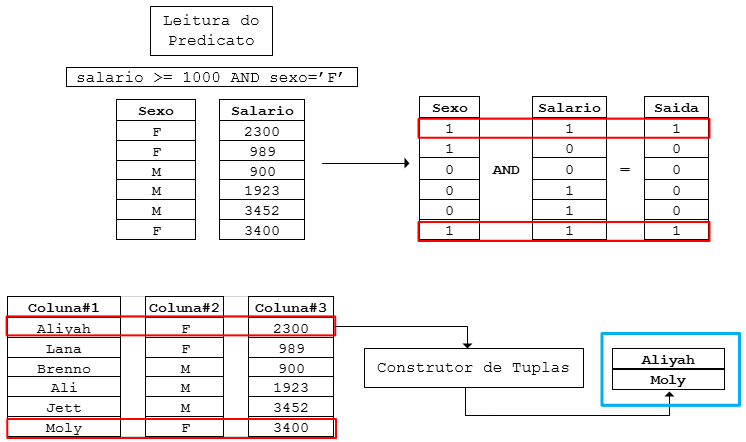
\includegraphics[width=14cm]{lm}
	\caption{Tuplas reconstruídas a partir da \textit{Late Materialization}}
	\label{fig:lm}
\end{figure*}

Na LM, ou materialização tardia, é analisado primeiro o predicado e verificado quais valores atendem a esse predicado em cada coluna. 
No caso da SQL acima primeiro seria analisado o predicado de seleção, nesse caso \texttt{WHERE salario >= 1000 AND sexo='F'}, e então 
através do operador lógico AND seria possível retornar a posição dos atributos que satisfazem essa seleção, para então 
construir a tupla a partir do predicado de projeção somente com o atributo \textit{nome}. Em suma, apenas após ter a posição de cada atributo é que a tupla é construída, descartando a reconstrução de tuplas que seriam posteriormente descartadas. A Figura \ref{fig:lm} apresenta o resultado após a construção das tuplas na LM.

% inserir subfigure com tuplas

\subsection{Particionamento Vertical}

Considerada a técnica mais simples para implementar um banco colunar, esta técnica 
realiza a partição dos dados de forma que cada atributo de uma entidade seja armazenado 
em uma tabela de duas colunas contendo o par <chave/índice, valor do atributo> \cite{khoshafian1987query}.

% inserir figura de particionamento vertical

A Figura \ref{fig:vertical} mostra que é possível desmembrar o esquema relacional da Figura \ref{fig:regs} em colunas de atributos -- foram desmembrados os atributos \textit{nome, sexo} e \textit{salario}. 
No momento em que uma consulta analítica é realizada, não serão processados dados além 
dos de fato requeridos e nenhum dado é perdido pois ainda haverá referência entre os atributos 
através das chaves.

\begin{figure*}[htpb]
	\centering
        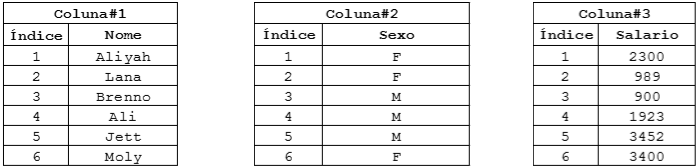
\includegraphics[width=\textwidth]{vertical}
	\caption{Implementação do modelo colunar utilizando particionamento vertical}
	\label{fig:vertical}
\end{figure*}

Essa abordagem é a mais simples de se implementar, pois nenhuma mudança é feita 
na codificação do banco de dados, sendo que a única alteração necessária está a nível 
da aplicação responsável por executar as consultas, mudando a lógica de acesso aos dados. Isso torna prático para empresas a 
mudança entre a estratégia relacional e a colunar, pois torna possível o uso de um mesmo 
SGBD como DW.

Ao mesmo tempo que essa implementação traz praticidade na migração de dados, ela não difere 
muito da abordagem relacional no que concerne ao desempenho. Em Abadi \cite{abadi2008query} 
é mostrado que adaptar dados de um esquema relacional utilizando particionamento vertical não 
trouxe melhoras no desempenho das consultas. Foi verificado que o custo de junções para unir 
as colunas é alto conforme a quantidade de atributos selecionados aumenta e não foi possível 
usufruir eficientemente da compressão de dados.

\subsection{Modificação na Camada de Armazenamento}

A segunda abordagem para implementar um sistema colunar consiste em já modificar o armazenamento do banco. Essa técnica não altera a parte 
lógica da modelagem do banco, mas a camada física alterando o armazenamento de 
linha por linha para coluna por coluna. Nessa implementação as chaves não precisam ser 
repetidas como na abordagem anterior, na qual a primeira coluna de cada tabela 
consistia no valor de chave da cada atributo. O \textit{i-ésimo} valor de atributo 
de uma coluna estará associado ao \textit{i-ésimo} atributo das demais colunas e 
não é desperdiçado espaço em disco com as chaves.

Neste método a reconstrução de tuplas é realizada antes da execução da consulta de fato. Como apenas um determinado número de atributos precisa ser acessado, estes são combinados seguindo a lógica que o \textit{i-ésimo} atributo de uma coluna está relacionado com o \textit{i-ésimo} atributo das demais. Aqui tem-se uma vantagem no modelo orientado a linhas, por este já armazenar as sob o formato de linhas e não precisar armazenar os dados em ordem.

\subsection{Modificação na Camada de Armazenamento e Particionamento Vertical}

A última, e melhor, abordagem consiste em modificar a camada de armazenamento do banco de dados e a aplicação que processa as consultas \cite{stonebraker2005c, boncz2005monetdb}, assim o processador pode manter os dados sob a forma de colunas sem precisar unir as colunas e construir tuplas. Uma vantagem óbvia desta técnica é a eliminação da reconstrução de tuplas e com isso menos dados precisam ser previamente movimentados, diminuindo 
o tempo de processamento.  

\section{Compressão de Dados}

Uma característica marcante de um SGBD colunar é a alta possibilidade de compressão de dados. 
Existem diversas formas de comprimir os dados, porém deve-se ater ao fato de 
que o tempo de compressão e descompressão não deve afetar significativamente o processamento 
dos dados no SGBD. Para tal, uma solução é utilizar métodos que consigam operar sob os dados 
ainda comprimidos -- ainda nesta seção são apresentados alguns dos algoritmos utilizados para 
compressão em banco de dados.

Como exemplo, apenas ilustrativo, de como os dados em um sistema colunar podem ser comprimidos de forma mais 
eficiente que em um relacional, considere a entidade \textit{usuário} a seguir, com os 
atributos \textit{id, nome, idade} e \textit{sexo}. A primeira coluna corresponde aos índices utilizados no banco. 

\begin{verbatim}
    1: 0, Bruno, 50, M
    2: 10, João, 23, M
    3: 20, Maria, 30, F
    4: 90, Ana, 23, F
    5: 78, Gabriel, 23, M
\end{verbatim}

Um banco relacional armazena estes atributos da forma como foram apresentados acima. 
Considerando o armazenamento colunar, os mesmos dados seriam armazenados da seguinte forma: 

\begin{verbatim}
    1: 0, 2: 10, 3: 20, 4: 90, 5: 78
    1: Bruno, 2: João, 3: Maria, 4: Ana, 5: Gabriel
    1: 50, 2: 23, 3: 30, 4: 23, 5: 23
    1: M, 2: M, 3: F, 4: F, 5: M
\end{verbatim}

Note que fica mais claro que como os atributos são armazenados em uma coluna com chave e valor 
existirão mais chances de repetição de valores em uma mesma coluna. Os atributos \textit{idade} e 
\textit{sexo} se repetem para alguns registros, possibilitando assim compressão destes dados. 
Comprimindo estas repetições o nosso modelo é armazenado da forma: 

\begin{verbatim}
    1: 0, 2: 10, 3: 20, 4: 90, 5: 78
    1: Bruno, 2: João, 3: Maria, 4: Ana, 5: Gabriel
    1: 50, 2, 4, 5: 23, 3: 30
    1, 2, 5: M, 3, 4: F
\end{verbatim}

Westmann et al. \cite{westmann2000implementation} consideram que os métodos de compressão em um banco de dados devem ser capazes de se aplicar 
no banco como um todo, bem como em uma tupla ou a cada atributo de tupla, e serem rápidos em processamento quando há casos em que seja 
necessário realizar descompressão.

O primeiro método consiste em comprimir a representação de valores inteiros, baseado no algoritmo \textit{null supression} \cite{westmann2000implementation, roth1993database}. A ideia é descartar zeros na representação de um inteiro de quatro bytes, por exemplo, 
ao invés de se representar o número 10 da forma '00000000000000000000000000001010', seriam utilizados apenas quatro bits, '1010'. É 
necessário entretanto guardar a informação de quantos bits são utilizados para armazenar um número e em alguns casos também é preciso 
armazenar um bit a mais para o sinal do inteiro. Esse algoritmo pode ser utilizado para comprimir o tamanho de strings no banco 
quando estas são representadas pelo tipo VARCHAR, visto que para esse tipo de dado o tamanho também é armazenado devido a possibilidade 
deste variar.

Um método bastante empregado é a Codificação por Dicionário. Nele atributos que possuem um padrão fixo, por exemplo, os números primos de 
3 a 19 (3, 5, 7, 11, 13, 17, 19), podem ser representados por um dicionário de 3 bits. Este algoritmo pode ser utilizado para compressão 
de valores NULL, considerando-o como um possível valor no padrão.

Abadi, Madden e Ferreira \cite{abadi2006integrating} utilizam a compressão por dicionário e uma variação do algoritmo \textit{null supression} para implementar o banco de dados C-Store e ainda apresentam dois outros métodos. O primeiro é o \textit{run-length}, que pode ser bem aproveitado 
em bancos colunares quando atributos são repetidos sequencialmente e possuem pouca variação. Ele consiste em contar o número de vezes no qual 
um valor é repetido utilizando a tripla (valor, posição inicial, tamanho). 
% Um exemplo é ilustrado na Figura A com o atributo \textit{especialização}.



% inserir uma imagem run length com graduação, mestrado, doutorado.

O último método apresentado pelos autores é a Codificação por Vetor de Bit, bastante útil quando uma coluna possui número limitado 
de possibilidades, como linguagens de programação dentro de um dado paradigma ou estados do Brasil. Uma string de bits representa a 
ocorrência do valor de atributo, onde '1' representa a ocorrência naquela posição e '0' a não ocorrência. Como exemplo, uma coluna com os 
valores {M M F M F F M} podem ser representados pela cadeia de bits 1 1 0 1 0 0 1 para o valor M, e 0 0 1 0 1 1 0 para F.

Em suma, ao implementar um banco colunar tanto a aplicação deve ser capaz de entender e conseguir recuperar informações mesmo comprimidas, como a modificação da camada de armazenamento deve ser implementada tal que se possa usufruir de algum método de compressão. Caso contrário um 
dos principais diferenciais de modelos colunares não será explorado e poderá não haver impacto no desempenho quando trabalhado com uma 
grande massa de dados, como é a realidade de empresas.
